\documentclass{ximera}
   
%% You can put user macros here
%% However, you cannot make new environments

\listfiles

\graphicspath{{./}{firstExample/}{secondExample/}}

\usepackage{tikz}
\usepackage{tkz-euclide}
\usepackage{tikz-3dplot}
\usepackage{tikz-cd}
\usetikzlibrary{shapes.geometric}
\usetikzlibrary{arrows}
\usetikzlibrary{decorations.pathmorphing,patterns}
\usetkzobj{all}
\pgfplotsset{compat=1.13} % prevents compile error.

\renewcommand{\vec}[1]{\mathbf{#1}}
\newcommand{\RR}{\mathbb{R}}
\newcommand{\dfn}{\textit}
\newcommand{\dotp}{\cdot}
\newcommand{\id}{\text{id}}
\newcommand\norm[1]{\left\lVert#1\right\rVert}
 
\newtheorem{general}{Generalization}
\newtheorem{initprob}{Exploration Problem}

\tikzstyle geometryDiagrams=[ultra thick,color=blue!50!black]

\usepackage{mathtools}
   
\title{Tank Draining}
   
\begin{document}
   
\begin{abstract}
An experiment involving a draining tank.
\end{abstract}
   
\maketitle
   
\section*{Tank Draining} 
 
This activity is intended to illustrate how the modeling process with differential equations is used to solve a practical problem.  Beginning with physics principles like conservation of mass and energy and a few simplifying assumptions, a differential equation is derived to describe the draining of water from a container.  After solving the differential equation, students can predict the time necessary to drain the container and then check this prediction with a simple experiment using readily available materials.
 
\subsection*{Overview of the Model}
 
Consider an open cylindrical tank of height $h_o$ that is filled with water or some other freely flowing liquid.  The cross sectional area is a constant value of $A$ and a small circular hole near the bottom has a much smaller area $a$. 
 
\begin{image}
 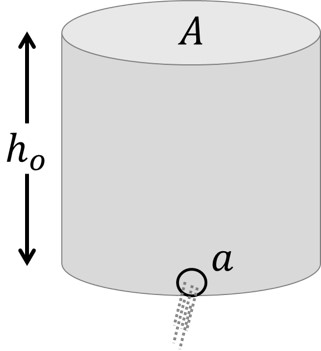
\includegraphics[height=1.5in]{drainingTank1.jpg}
\end{image}
 
When the water is allowed to flow from the hole, the tank will eventually drain until the water level reaches the hole.  Our goal is to predict how long this draining process will take.  We will try to measure the draining time, which we will define as the elapsed time from when the water is allowed to flow out until the water level reaches the top of the hole.  Before outlining the derivation below, make a prediction about what parameters impact the draining time.  Make a list on paper of every variable upon which the draining time will depend.
Examine your list.  Did you include parameters like air pressure, the density of the fluid, or the shape of the small hole?  Did you include $A$, $a$, and $h_0$?  If so, what would an increase in these parameters do to the draining time?  As the water drains, will the flow rate remain constant?  Now that you have written down your predictions, let’s derive a model for this process.  When the model is derived, return to your list to check it.

Before developing a full model, reflect on your physical experience and/or intuition with draining containers to answer the following question.  

\begin{question}\label{quest:guessGraphTank}
Which of the following graphs best predicts how the height of water in this tank will change with time?
 
%\begin{multipleChoice}
%\choice
%{\begin{image}
% \includegraphics[height=1.5in]{Plot1.png}
%\end{image}}
%
%\choice[correct]
%{\begin{image}
% \includegraphics[height=1.5in]{Plot2.png}
%\end{image}}
%
%\choice
%{\begin{image}
% \includegraphics[height=1.5in]{Plot3.png}
%\end{image}}
%
%\choice
%{\begin{image}
% \includegraphics[height=1.5in]{Plot4.png}
%\end{image}}
%
%\end{multipleChoice}



Expand for discussion.
 
\begin{expandable}
    The first option is incorrect.  This plot indicates that the height of water is changing most rapidly in the middle of the draining process and slowly in the beginning and end.  This is not the observed behavior of the height of water in a draining tank.
    
     \textbf{The second option is correct}.  This plot correctly indicates the observed behavior.  Notice that the height of water in the tank changes most rapidly in the beginning.  This is because when the water level is the highest, the flow rate out will be the greatest.  The flow rate out diminishes as the height of water is reduced.
     
     The third option is incorrect.  This plot indicates that the water level will decrease at a constant rate throughout the draining process.  This is not the observed behavior, because the flow rate of water actually depends on the height of water in the tank.
     
     The fourth option is incorrect.  This plot suggests that the height of water will change slowly at the beginning and will change more rapidly at the end.  This is not the observed behavior of such a system.  
     
 \end{expandable}
 
 \end{question}
 
\subsection*{Model Derivation}
 
As with many modeling problems leading to differential equations, it is helpful to begin with a generic balance equation:
$$\mbox{flow in}-\mbox{flow out}+\mbox{generation}-\mbox{destruction}=\mbox{accumulation}$$
 
While this principle can be applied to many different quantities for a defined system, we can immediately apply it to the mass of the water in the tank.  This equation can be called a rate equation because each of the terms refer to a rate (rate of flow in, rate of destruction, rate of accumulation, etc.)  Can you see which of the terms in this generic equation can be crossed off? 
 
From physics, we recall that mass – just like energy and momentum – is a conserved quantity under normal circumstances.  This means that it cannot be generated or destroyed.  Furthermore, we note that water only flows out of, not into, the tank during the draining process.  This leaves us with:
$$-\mbox{rate of mass flow out}=\mbox{rate of accumulation of mass}$$
We also recognize that the density of water (mass per unit volume) is constant.  Thus, since it is easier in our experiment to describe changes in volume and the rate of flow of volume, we can instead write:
$$-\mbox{rate of volume flow out}=\mbox{rate of accumulation of volume}$$
We can now incorporate both of the areas in the diagram above.  First, we recognize that the rate of volume flow out of the tank is equal to the velocity of the water through the small hole multiplied by the area $a$.  Second, we take note of the relationship between the volume, the height, and the cross sectional area of the cylindrical tank.  The rate of accumulation or depletion of volume is equal to the rate of change in height multiplied by the cross sectional area.  Our balance equation now becomes:
$$-a(\mbox{velocity out})=A\frac{dh}{dt}$$
 
Observe that the units of this equation are still a rate of change of volume (length cubed per time).  It is helpful that we now have the time rate of change of height in our equation.  We can and will estimate both of the areas.  Yet, we do not yet have an idea of the velocity of the water coming out of the small hole.  Our derivation so far relied on the principle of conservation of mass.  To find the velocity out, we will employ the principle of conservation of energy.
For this system, the principle of conservation of energy leads us to Bernoulli’s Equation, which is an important relationship between pressure, velocity, and height of a flowing fluid:
$$P+\frac{1}{2}\rho V^2+\rho gh=\mbox{constant}$$
 
Here, $P$ is the pressure, $\rho$  is the density, and $V$ is the velocity of the fluid.  The gravitational constant $g$ and the height $h$ of the fluid, relative to some reference point, also appear.
The units of each term in this equation are pressure, which is force per unit area.  However, it is also helpful to realize that this is also energy per volume.  Can you see this if we note that energy is force times distance and volume is area times another distance?  Bernoulli’s equation shows us how energy, though conserved overall, can be transferred in different categories.  A fluid may have energy due to its pressure, due to its velocity (kinetic energy), and due to its height (potential energy).  All three of these ways of having energy are included in this equation on a per volume basis.  Now, considering two points in the system, we can use this relationship to specify the velocity of water flowing out of the small hole. 
\begin{image}
 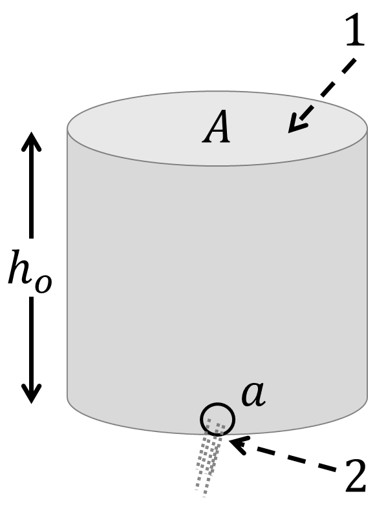
\includegraphics[height=1.5in]{drainingTank2.jpg}
\end{image}
 
Point 1 is at the very top of the water in the tank.  Point 2 is on the water as it leaves the small hole.  Bernoulli’s equation is applied to these two points:
 
$$P_1+\frac{1}{2}\rho V_1^2+\rho gh_1=P_2+\frac{1}{2}\rho V_2^2+\rho gh_2$$
 
Since both points are open to the atmosphere, they are at almost exactly the same pressure.  The small difference in height does not produce a very different air pressure.  For this reason, $P_1$ and $P_2$ can be crossed off together.  Since the density  of water does not change at all, it can be cancelled from all of the remaining terms.  Rearranging gives the following:
 
$$V_2^2-V_1^2=2g(h_1-h_2)$$
 
Further simplification is possible if we neglect $V_1^2$.  This is defensible because $V_2$ is much larger than $V_1$ since the cross sectional area of the tank $A$ is – in most cases – significantly larger than the area of the small hole.  The square of $V_1$  must therefore be smaller, relatively speaking, than the square of $V_2$. Water will be moving much more quickly out of the small hole than the movement of the top surface of the water.  We can replace the different in heights between two points with $h$, which is the height of water above the small hole at any point in time.  This can now be written as:
 $$V_2=\sqrt{2gh}$$
  
 It is evident that as the tank drains, the velocity of the water draining out will decrease toward zero since the height of the water is decreasing toward zero.  When we conduct the experiment, we expect that the fastest stream of water will be seen at the very beginning.  Having solved for the velocity at Point 2, which is the ``velocity out" in the simplified balance equation above, we can now put everything together:
 $$A\frac{dh}{dt}=-a\sqrt{2gh}$$
 Since $A$, $a$, and $g$ are all constant in our model of the cylindrical tank, we can lump all the constants together as $k$ and write:
  
 $$\frac{dh}{dt}=-k\sqrt{h},\quad \text{where}\quad k=\frac{a}{A}\sqrt{2g}$$
 
It is instructive to check the units of this differential equation, which are length per time since it gives us the rate of change of height.  Note that the units of the constant $k$ are $\sqrt{m}/s$.  We have now derived a differential equation for the height of the fluid in the tank by using principles from physics and some appropriate simplifications. 
Separation and integration leads us to a solution for water height as a function of time:
 
$$\int\frac{dh}{\sqrt{h}}=\int -k\,dt$$
$$2\sqrt{h}=-kt+C$$
Here we specify the constant of integration in terms of the initial height at $t=0$.
$$C=2\sqrt{h_0}$$
Rearrangement gives the solution of our differential equation:
$$h=\left(\sqrt{h_0}-\frac{kt}{2}\right)^2$$
From here, we can determine the time necessary for the tank to drain, because this is when $h=0$.
$$t_f=\frac{2\sqrt{h_0}}{k}$$
If we substitute for the constant $k$, we find that the final time is
$$t_f=\frac{A}{a}\sqrt{\frac{2h_0}{g}}$$

Note that, according to our assumptions in this model, no other factors will impact the draining time: not the air pressure, the density of the fluid, or the shape of the drain hole.  In fact, the drain hole and the cross section of the tank could be circular, square, or any other shape.  We only require that the area of the cross section of the tank remain constant.  For instance, this model would correctly predict the time to drain a cube shaped container.
One other interesting aspect of the mathematics here is evident when one studies the solution to the differential equation, which is parabolic in form.  Notice that if the time exceeds the calculated draining time, the solution predicts that the height of the water would again increase.  This is an aphysical (not real) prediction, because once the tank drains completely the height of the fluid will stay at exactly zero.  Examine the differential equation and note that $h=0$ is a stable (equilibrium) solution.
 
Before conducting an experiment to check the accuracy of this model, let’s examine your predictions of which parameters impact the draining time.  Consider a tank with cross sectional area $A$ and hole area $a$ with an initial height $h_o$.  What will happen to the draining time in each of the following cases?  

\begin{question}\label{quest:guessGraph}
If $A$ is doubled, the draining time will…
\begin{multipleChoice}
\choice {Shorten by some amount that cannot be specified}
\choice {Shorten by half}
\choice {Remain unchanged}
\choice [correct] {Lengthen to twice its initial value}
\choice {Lengthen by some amount that cannot be specified}
\choice {Change in some other way}
\end{multipleChoice}
\end{question}
Expand for discussion.
\begin{expandable}
    In the equation for $t_f$ above, the draining time is directly proportional to the cross sectional area of the tank $A$.
 \end{expandable}

\begin{question}\label{quest:guessGraph}
If $h_o$ is doubled, the draining time will…
\begin{multipleChoice}
\choice {Shorten by some amount that cannot be specified}
\choice {Shorten by half}
\choice {Remain unchanged}
\choice {Lengthen to twice its initial value}
\choice {Lengthen by some amount that cannot be specified}
\choice [correct] {Change in some other way}
\end{multipleChoice}
\end{question}
Expand for discussion.
\begin{expandable}
    While a larger initial height will cause the draining time to increase, it is interesting to note that the dependence is not directly proportional in the same way as it was with cross sectional area $A$.  Doubling the initial height will cause the draining time to be just over $41\%$ larger.  Note that the initial height is inside the square root in the equation for $t_f$ above. 
 \end{expandable}
 
\subsection*{Tank Draining Experiment}
 
To conduct your own experiment, you should assemble the following near a sink or an outside location:
\begin{enumerate}
\item
A plastic bottle or other container that has a constant cross section.  Most containers, such as a two-liter soda bottle, would work. Ideally, the bottle will be at least partially transparent to see the water level.  The top should be open to the atmosphere to prevent a vacuum.  You could even choose to cut the top of the bottle off with scissors to make measuring easier, although this is not required.  The example demonstrated here is done with a plastic vinegar bottle shown at right.  Note that we will only allow the water to drain through the region with a constant cross section (just above the label to the hole punctured just below the label).
\item
A pushpin that can be used to poke a small hole for the drain.
\item
A pencil or pen that can be used to widen the drain hole.
\item
A ruler with fine gradations, preferably with metric units such as centimeters.
\item
A stopwatch, clock, or phone to record the drain time
\end{enumerate}
 
\begin{image}
 
\includegraphics[height=1.5in]{appleCider.jpg}
\end{image}
 
Use the pushpin to start the hole, then widen it with the pencil or pen.  Try to make the whole as close to circular as possible.  The diameter of a pen, less than $7mm$, is an appropriate size to conduct a first experiment, but you could do more experiments after incrementally widening the hole.  Mark the place on the bottle for the initial water level.  Plan to drain only the region with a constant cross sectional area.  (Our simple model was not derived for an area A that depended on the height.)  Measure this initial height $h_o$ from your water mark down to the top of the small hole.  Also make your best estimate of the diameter of the container and the small hole in order to calculate the areas $A$ and $a$.  If using a container with something other than a circular cross section, calculate the area according to that geometry.  Use all of these parameters to estimate the time to drain $t_f$.  It is recommended that you convert all parameters to a common unit such as meters and use $g=9.81$ $m/s^2$.  As you fill the bottle to the line, you could leave the pen stuck in the bottle or keep your finger over the hole.  Make your best estimate of the draining time and stop the timer the moment the water level reaches the top of the hole.  As the tank drains, recall our prediction that the velocity of the stream would be largest at the beginning.  Draining will slow down greatly as the water height diminishes. 
 
\begin{image}
 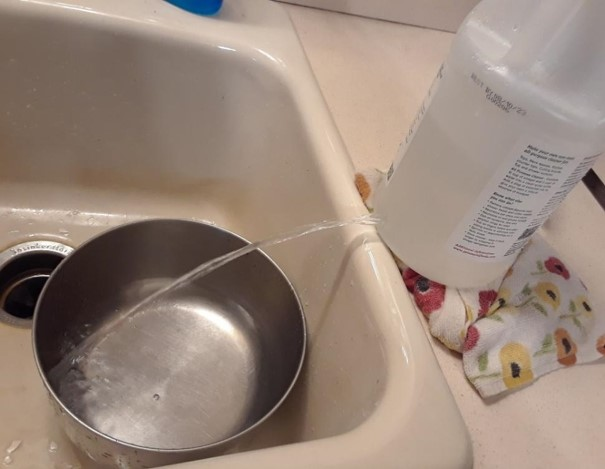
\includegraphics[height=1.5in]{sink.jpg}
\end{image}
 
In this example, the initial height was measured to be $h_0=12.5 cm$.  The hole diameter was approximated to be about $0.62 cm$, giving a hole area $a=3.02\times 10^{-5} m^2$.  The container diameter was about $11.2 cm$, giving a cross sectional area $A=9.85\times 10^{-3} m^2$.  Note that $A$ is over $300$ times larger than $a$, supporting our previous assumption that $V_2$ is much larger than $V_1$.  The lumped constant is thus calculated to be $k=0.0136 m/s$ and the draining time is predicted to be about $52$ seconds.  See the predicted trajectory of the water level vs. time in the plot below.  When the experiment was carried out, it actually took $56$ seconds for the tank to drain.  Thus, the observed time was almost $8\%$ longer than the predicted time.  This is not bad.  Is your estimate also slightly shorter than the actual draining time?
 
\begin{image}
 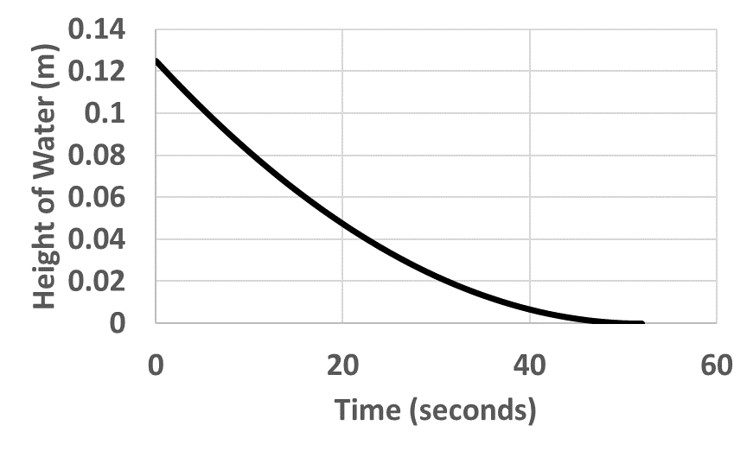
\includegraphics[height=1.5in]{drainingTank3.jpg}
\end{image}
 
\subsection*{Sources of Error}
 
It is instructive to consider what sources of error may have been most important in our derivation and measurements.  List what assumptions you believe may have been most dubious.  Are all of your measurements accurate?  Below, we will examine each major assumption and also estimate possible measurement errors in our analysis.  When possible, we can predict whether a flaw in our model would cause an overestimate or an underestimate in draining time.
 
\begin{enumerate}
    \item
    We assumed that the liquid water was freely flowing.  Specifically, we assumed that the viscosity of our fluid was negligible.  One can imagine the importance of viscosity in the case of less freely flowing substances like honey or molasses.  Furthermore, it is possible that rough edges near our small drain hole – crudely poked with a pen or pencil – could have inhibited the flow of water, slightly slowing the draining process.  A fluid’s viscosity causes resistance to flow that – to a certain extent – lessens the overall conversion of potential to kinetic energy because some of that energy goes into internal energy (essentially heating the fluid and its surroundings).  In the case of water, it is likely that the velocity flowing out of the tank was overestimated by a small amount – likely a couple percent.  Thus, for this reason, the model used here would tend to underestimate the draining time.  In our example above, we might have been a bit closer to the correct answer.
    \item
    Neglecting the term $V_1^2$ seemed reasonable during the derivation, and allowed us to further simplify Bernoulli’s Equation:
    $$V_2^2-V_1^2=2g(h_1-h_2)=2gh$$
    Instead of neglecting this velocity of the top surface of the water, we could have chosen to relate it to the other velocity of the water at the drain hole.  Recall that our balance equation had led to the following relationship:
    $$-a\mbox{(velocity out)}=A\frac{dh}{dt}$$
    We recognize that the "velocity out" is $V_2$ and that $-\frac{dh}{dt}$ is equal to $V_1$, since it is the rate of change of the height of the water.  For that reason, we recognize that $V_1=\frac{a}{A}V_2$.  This enables us to write Bernoulli's equation as:
    $$V_2^2-\left(\frac{a}{A}V_2\right)^2=2gh$$
    In contrast to our previous simplified result $V_2=\sqrt{2gh}$, we now arrive at:
    $$V_2=\sqrt{\frac{2gh}{1-\left(\frac{a}{A}\right)^2}}$$
    However, here we realize that our previous simplification was more than warranted.  As noted in the example above, the area $a$ is more than three hundred times smaller than $A$, which means that denominator $1-\left(\frac{a}{A}\right)^2$ is very nearly $1$, making the difference negligible.  Other assumptions and errors in measurement likely dwarf this error.
    \item
    Measurement error may also have been significant.  For instance, we measured the small drain hole with a ruler, approximating the diameter to be about $0.62 cm$.  Given its small size, this is a difficult estimate to make with only a ruler.  Run the calculation again to see that if we had been just $5\%$ off in this estimate of this diameter, the draining time would vary by almost $10\%$, or about $5$ seconds.  This is a substantial change in the overall prediction resulting from a very modest difference in our measurement.  Other measurement errors are possible including the other two lengths and the recorded time, but these are likely smaller than that caused by the measurement of the small hole.  This suggests that the accuracy of our modeling is highly dependent on the estimation of key distances, and measurement errors here could outweigh the effects of our assumptions regarding the physics of the model.  Measurement with calipers or the careful use of a drill bit to make the drain hole may be warranted to improve the accuracy of the model.
\end{enumerate}
 
 
\end{document}